\chapter{Conclusion}
\label{sec:conclusion}

\section{Global interpretations of results}

The analyses presented in Chapters~\ref{sec:bsm_H_to_tau_tau_analysis} and \ref{sec:H_A_to_4_tau_analysis}, although motivated by different physics, are complementary to one another in context of the type X \ac{2HDM}.
The limits on this phase space from the analysis discussed in Chapter~\ref{sec:bsm_H_to_tau_tau_analysis}, are studied using the \textsc{HiggsTools-1} framework~\cite{Bahl:2022igd}.
\textsc{HiggsTools} is a combination of the \textsc{HiggsBounds}, \textsc{HiggsSignals} and \textsc{HiggsPredictions} frameworks and these are used for the following purpose:

\begin{itemize}
\item \textsc{HiggsPredictions} is used to determine theory production cross sections and decay rates.
\item \textsc{HiggsBounds} is used to find direct bounds for searches for new particles.
\item \textsc{HiggsSignals} is used to find the bounds from shifts to the observed Higgs boson's properties.
\end{itemize}

\textsc{HiggsBounds} and \textsc{HiggsSignals} contain a database of results from all key measurements from the LHC, LEP and other colliders.
The result from Chapter~\ref{sec:bsm_H_to_tau_tau_analysis} is included in this database.
The widths of additional Higgs bosons and branching fractions calculated with \textsc{2HDECAY} for Chapter~\ref{sec:H_A_to_4_tau_analysis} are utilised for the scan of the type X 2HDM parameter space.
The cross sections used in each analysis scanned over is scaled to that of the model parameters by the \textsc{NeutralEffectiveCouplings} function in \textsc{HiggsPredictions}.
A 95\% CL limit is then tested on each point in the parameter space. \\

In the alignment scenario, the strongest bounds on the type X \ac{2HDM} at all mass points tested come from the analysis described in Chapter~\ref{sec:bsm_H_to_tau_tau_analysis}.
The limits determined for the $m_{\phi}$ equal to 100 and 200 GeV scenarios are overlayed onto the limits shown in Figure~\ref{fig:4tau_md} and shown in Figure~\ref{fig:4tau_md_hb}. \\

\begin{figure}[!hbtp]
\centering
    \subfloat[]{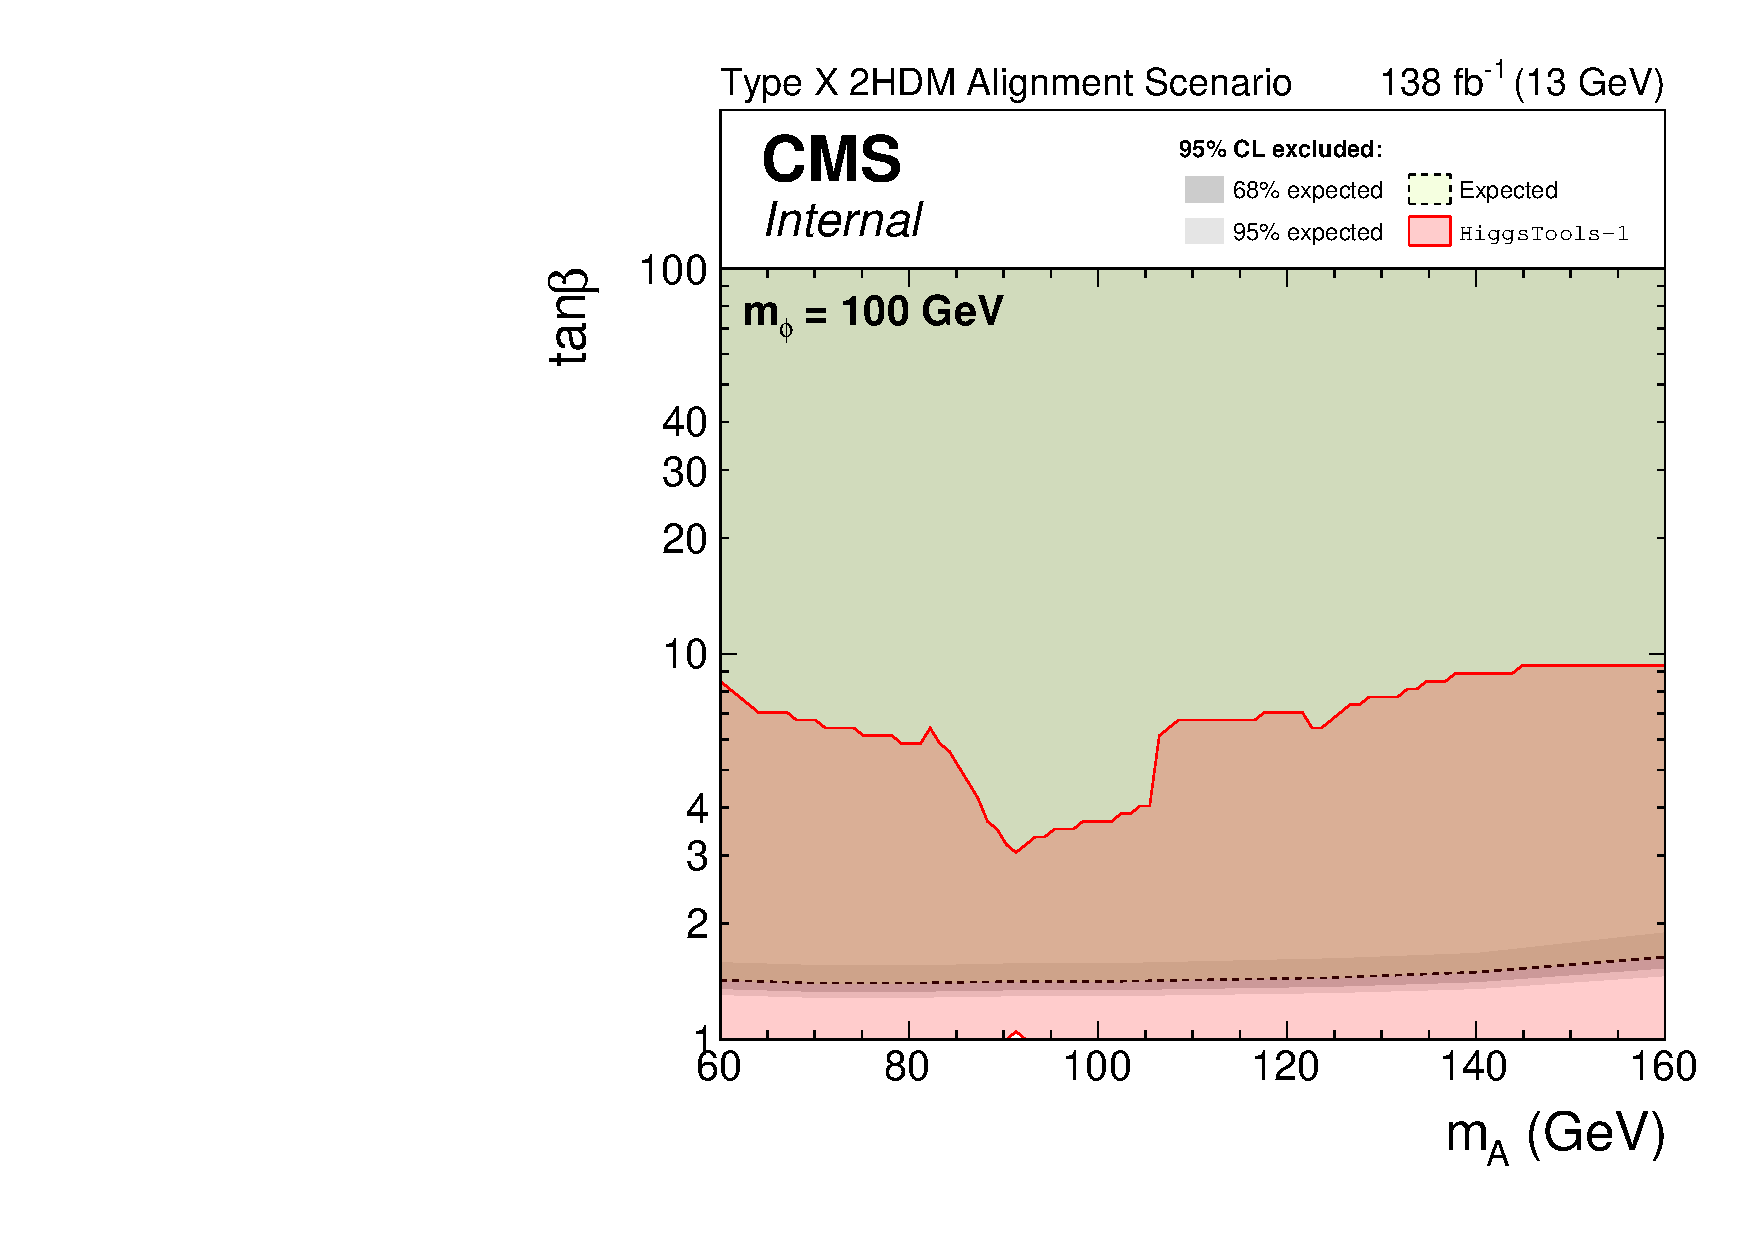
\includegraphics[width=0.7\textwidth]{Figures/md_mphi100_hb.pdf}} \\
    \subfloat[]{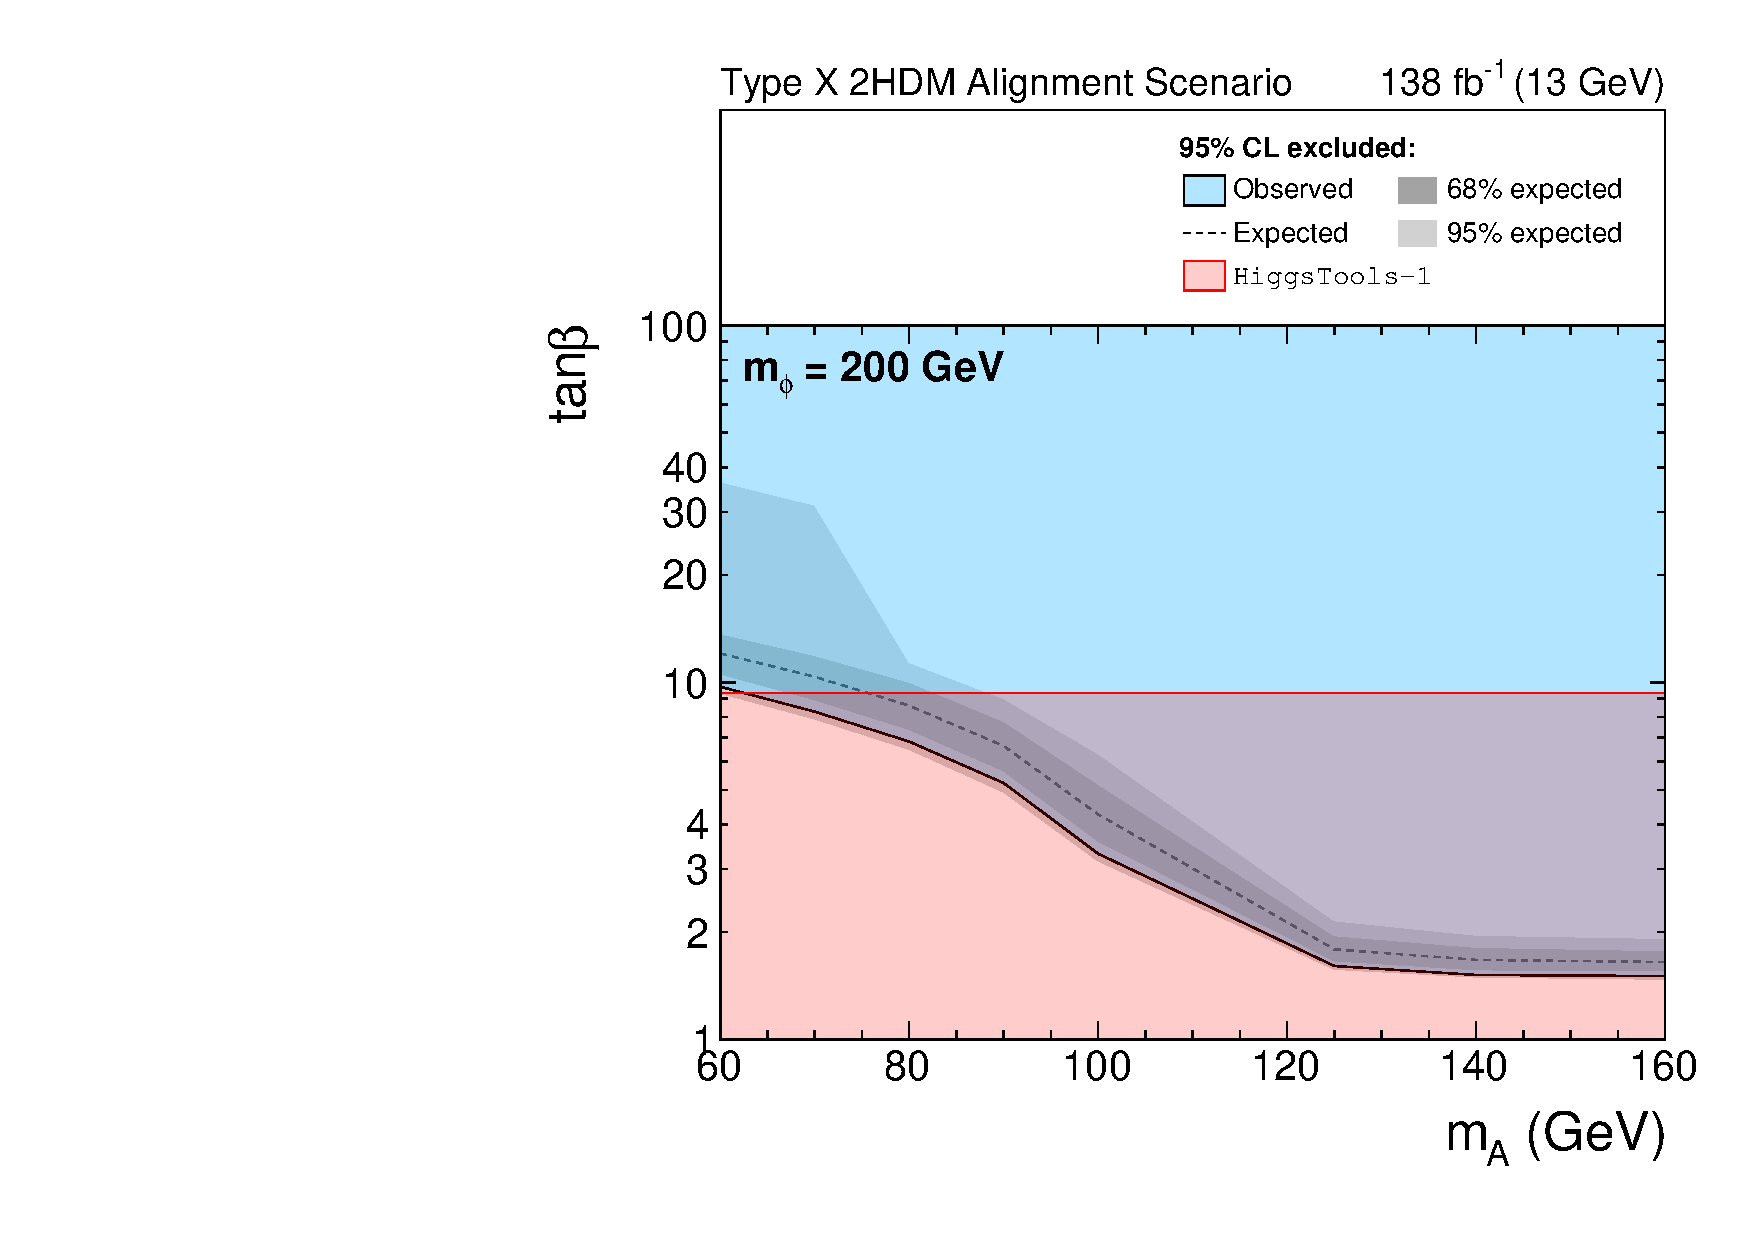
\includegraphics[width=0.7\textwidth]{Figures/md_mphi200_hb.pdf}} 
\caption{Expected and observed 95\% CL exclusion contours on the $m_{A}$-$\tan\beta$ phase space in the type X 2HDM alignment scenario for $m_{\phi}$ scenarios of 100 GeV (a) and 200 GeV (b). The exclusion limit only on background expectation is shown as a dashed black line, the dark and bright grey bands show the 68\% and 95\% intervals of the expected exclusion and the observed exclusion contour is shown by the blue area. The limit obtained by \textsc{HiggsTools} is shown in the red contour.}
\label{fig:4tau_md_hb}
\end{figure}

The previous strongest constraints on the type X \ac{2HDM} alignment limit parameter space comes from the analysis described in Chapter~\ref{sec:bsm_H_to_tau_tau_analysis}.
The exclusion limits are at low values of $\tan\beta$ only.
As $\tan\beta$ increases, the gluon fusion and b associated production modes are suppressed but the branching ratios of the additional Higgs bosons to $\tau$ leptons are enhanced.
Therefore, the exclusion limit represents a compromise between suppressed cross sections and enhanced branching ratios. 
The regions where the product is large enough for that parameter point to be excluded, happens at low $\tan\beta$.
In the type X \ac{2HDM}, the b associated production mode in negligible due to no enhancement of couplings to b quarks.
The mass hypotheses change the limit due to the non-flat nature of Fig.~\ref{fig:model_independent_limits}(a).
The limit in Fig.~\ref{fig:4tau_md_hb}(b) is flat as the the strongest constraint comes from the $\phi$(H) boson, and for an additional neutral \ac{CP}-even Higgs boson $\tan\beta \lesssim 10$ is excluded.
However, this is not the case for Figure~\ref{fig:4tau_md_hb}(a) where $m_{\phi}$ is lighter and the sensitivity is not always driven by the $\phi$(h) boson.
In particular, the limit on a 100 GeV resonance, from Fig.~\ref{fig:model_independent_limits}, is weakest due to the large Drell-Yan background and the local excess observed on top of this peak, and so effects from both additional neutral Higgs bosons are present.
Together, the exclusion limits from both analyses yield an almost complete coverage of the type X 2HDM alignment scenario within the mass range searched. \\

Next the affect of the \ac{BSM} searches and precision measurements of the \ac{SM} Higgs boson on the type X \ac{2HDM} model, outside of the alignment scenario is studied.
Bounds are again calculated with \textsc{HiggsTools}, however the constraints now come from \ac{SM} Higgs measurements as well as \ac{BSM} searches such as described in Chapter~\ref{sec:bsm_H_to_tau_tau_analysis}.
The bounds determined, overlayed with the results shown in Figure~\ref{fig:4tau_cosbma}, are shown in Figure~\ref{fig:4tau_cosbma_hb}. \\

\begin{figure}[!hbtp]
\centering
    \subfloat[]{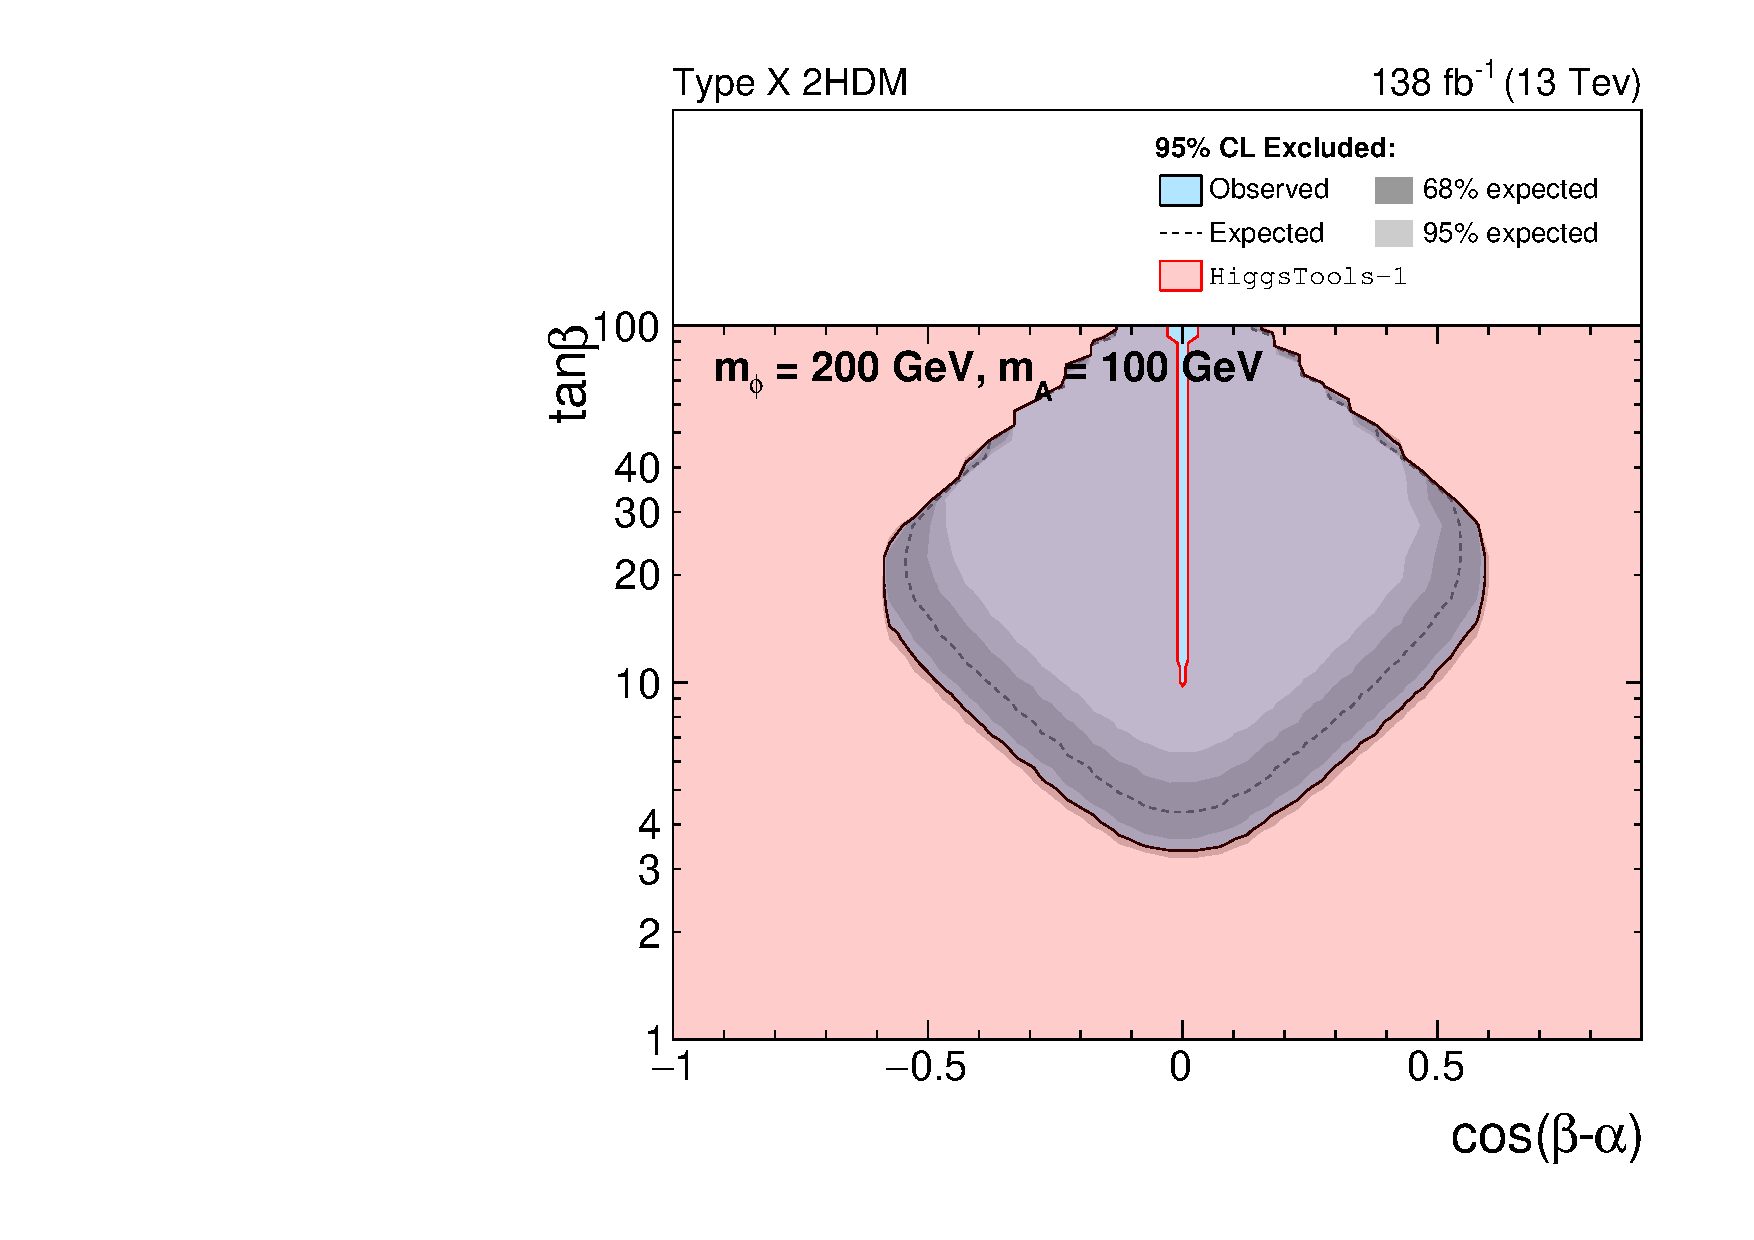
\includegraphics[width=0.65\textwidth]{Figures/csbma_phi200A100_hb.pdf}} \\
    \subfloat[]{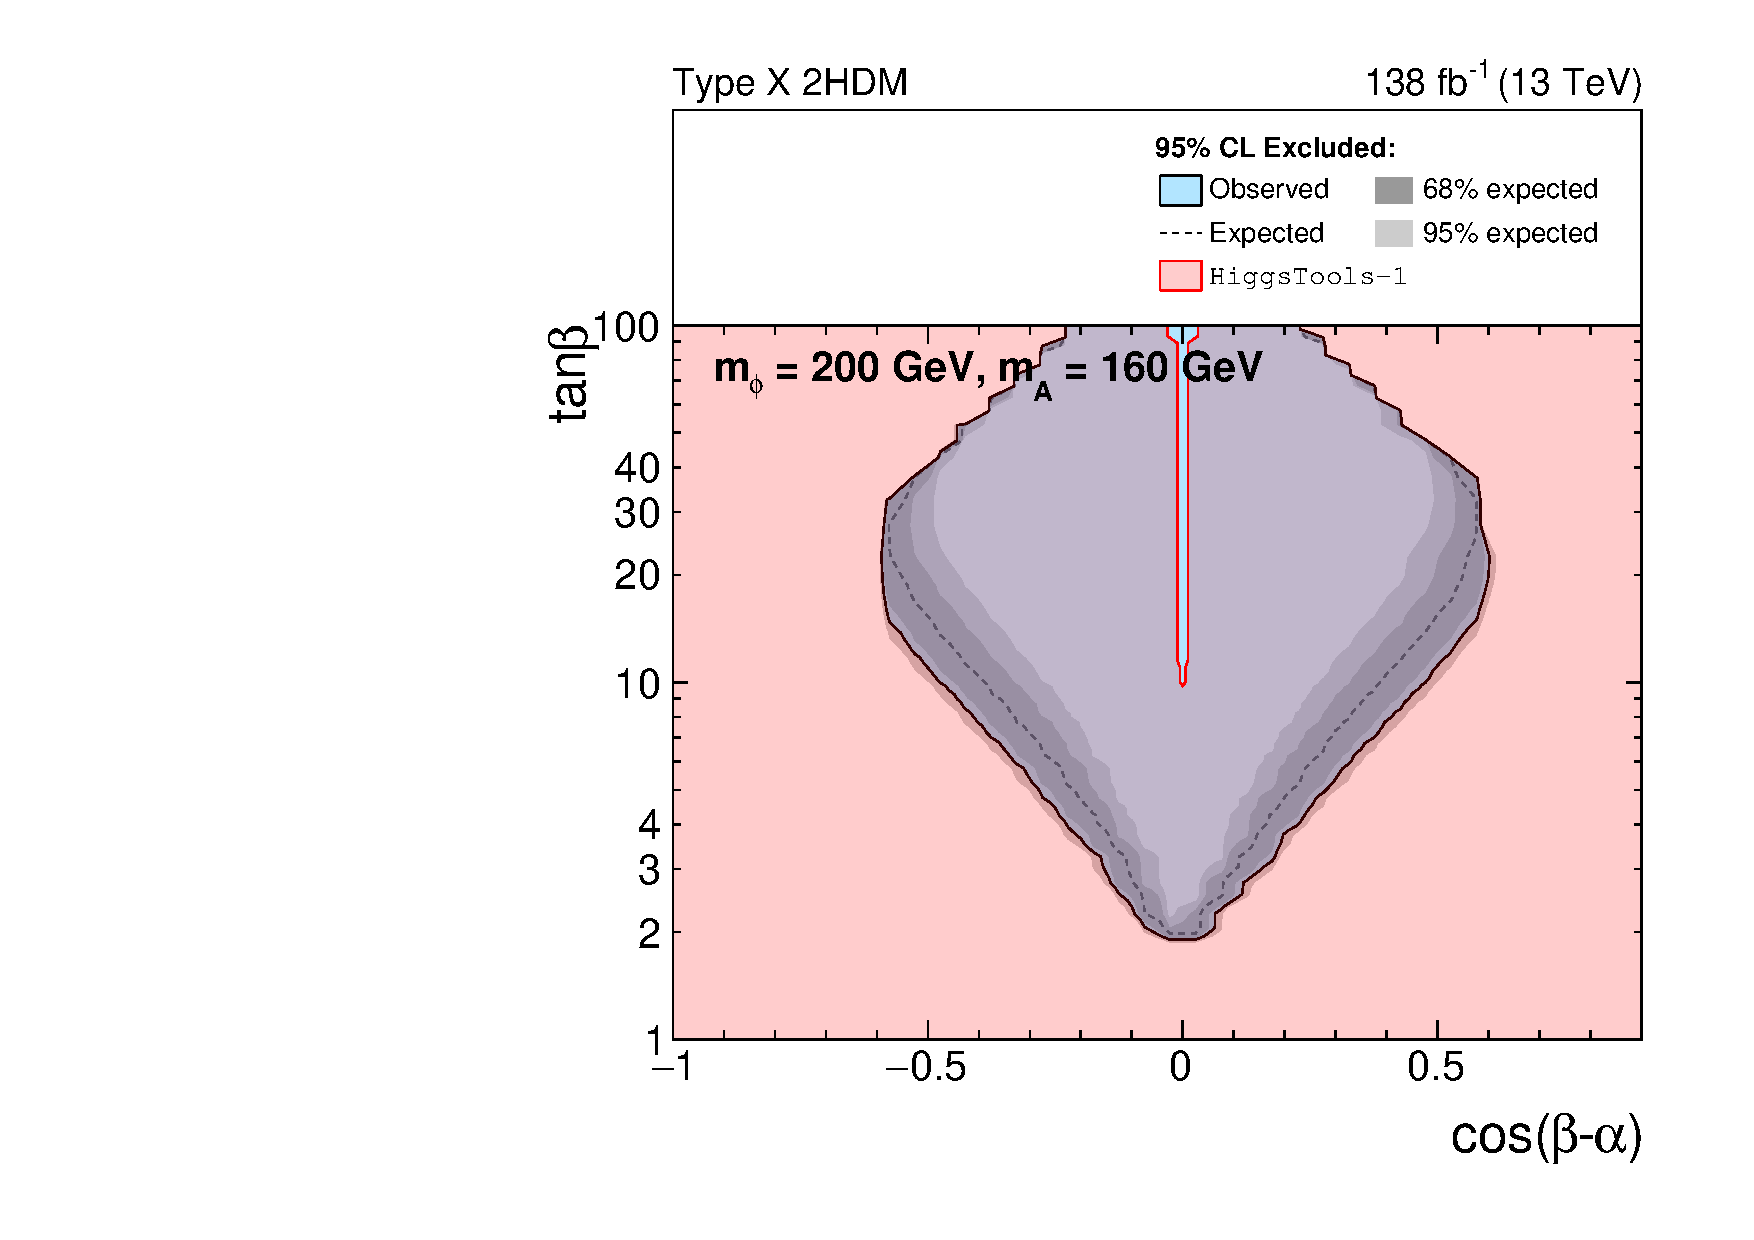
\includegraphics[width=0.65\textwidth]{Figures/csbma_phi200A160_hb.pdf}} 
\caption{Expected and observed 95\% CL exclusion contours on the $\cos(\beta-\alpha)$-$\tan\beta$ phase space in the type X 2HDM alignment scenario with $m_{\phi}$ equal to 200 GeV and $m_{A}$ scenarios of 100 GeV (a) and 160 GeV (b). The exclusion limit only on background expectation is shown as a dashed black line, the dark and bright grey bands show the 68\% and 95\% intervals of the expected exclusion and the observed exclusion contour is shown by the blue area. The limit obtained by \textsc{HiggsTools} is shown in the red contour.}
\label{fig:4tau_cosbma_hb}
\end{figure}

The limits determined from the Chapter~\ref{sec:bsm_H_to_tau_tau_analysis}, although stringent across values of $\cos(\beta-\alpha)$, are weaker than the constraints from the \ac{SM} Higgs boson when moving outside of the alignment limit.
They are nonetheless crucial in setting limits, when very close to or on the alignment limit.
The constraints from the \ac{SM} Higgs boson, significantly narrow the region allowed outside of the alignment limit and motivates the continued use of alignment scenarios for extended Higgs sector searches.
The combination of both \ac{BSM} and \ac{SM} Higgs boson results, prior to the work performed in Chapter~\ref{sec:H_A_to_4_tau_analysis}, leaves only a small strip of the phase space for new physics to exist.
However, the entirety of the phase space for the two mass points is excluded by the combination of the searches detailed in Chapters~\ref{sec:bsm_H_to_tau_tau_analysis} and \ref{sec:H_A_to_4_tau_analysis}, as well as precision measurement of the \ac{SM} Higgs boson.

\section{Summary}

This thesis has presented two analyses utilising the full Run 2 dataset collected by the \ac{CMS} experiment, from the 13 TeV proton proton collisions at the \ac{LHC}, targeting final states enriched in tau leptons.
The motivation for the searches presented in Chapter~\ref{sec:bsm_H_to_tau_tau_analysis} and \ref{sec:H_A_to_4_tau_analysis} are \ac{BSM} theories that attempt to resolve the theoretical issue of the hierarchy problem and the experiment tensions of the B anomalies and the g-2 anomaly.
The preceding chapters, act to motivate the new physics models that could potentially resolve these tensions, and the apparatus and methods used for the foundation of data taking and reconstruction required for the searches. \\

Chapter~\ref{sec:bsm_H_to_tau_tau_analysis} presents a search for two possible areas of new physics in the di-$\tau$ final states.
The first of these is a search for additional neutral Higgs bosons, motivated by the type II \ac{2HDM} of the \ac{MSSM}, as a consequence of a solution to the hierarchy problem.
This targets two production modes: gluon fusion and production is association with a b quark, with the latter dominant to a search for the \ac{MSSM} at higher values of $\tan\beta$.
No deviation is observed for the search for b associated production, that targets event categories that require a minimum of one b jet.
This makes it very difficult to coincide an \ac{MSSM} benchmark scenario with any gluon fusion signal.
The gluon fusion results yielded two small deviations from the \ac{SM} expectation, peaking at 100 GeV and 1.2 TeV with a local (global) statistical significance of 3.1$\sigma$ (2.7$\sigma$) and 2.8$\sigma$ (2.2$\sigma$) respectively.
The two excesses are present in the no b tag categories fit and are compatible across all decay channels and categories fit.
Good agreement between data and the background hypothesis is observed in the rest of the mass hypotheses.
Limits are set on the cross section of both production modes multiplied by the additional scalars decay to $\tau$ leptons and both of these vary from $\mathcal{O}$(10 pb) at 60 GeV to 0.3 fb at 3.5 TeV.
These results are also interpreted as exclusion limits in \ac{MSSM} benchmark scenarios.
In the $M_{h}^{125}$ scenario, values of $m_A < 500$ GeV are excluded, and in the remaining phase space as well as in the $M_{h, EFT}^{125}$ the strongest constraints on the phase space are set. \\

The second area of new physics that is searched for in Chapter~\ref{sec:bsm_H_to_tau_tau_analysis}, is a potential solution to the B anomalies, in vector leptoquarks.
The signal model searched for is a non-resonant t-channel interaction producing a di-$\tau$ final state, where the initial state is dominated by b quarks.
The best fit vector leptoquark is heavily constrained by the b tag categories where no deviation from the \ac{SM} expectation is observed.
It therefore can not be used to explain the deviations observed in the no b tag categories.
Limits on vector leptoquark phase space are set and constrain the regions allowed for an explanation to the B anomalies. \\

Chapter~\ref{sec:H_A_to_4_tau_analysis} details a search for an extended Higgs sector to explain the g-2 anomaly.
This can be done with type X \ac{2HDM} at high values of $\tan\beta$.
A different signal strategy is needed than in Chapter~\ref{sec:bsm_H_to_tau_tau_analysis}, due to the suppressed coupling between the additional neutral Higgs bosons and quarks in this model.
The preferred signal model here is the production of two additional neutral Higgs bosons via an off-shell Z boson.
At high values of $\tan\beta$, the branching fractions of the additional neutral Higgs bosons are dominated by di-$\tau$ pairs.
Therefore, the $\tau\tau\tau\tau$ final states are used to reconstruct this signal.
No significant deviation is observed from the background estimation.
Limits on the cross section multiplied by branching fractions are set and vary from 20 fb at the lowest mass hypothesis, to 1.4 fb at the highest mass hypothesis.
The results are interpreted in terms on the type X \ac{2HDM}, and it is found that the constraints from the \ac{SM} Higgs boson measurements limit the phase space to be very close to the alignment limit.
The alignment limit exclusions are found to exclude upwards of $\tan\beta$ approximately equal to 1.5, unless the $\PH \rightarrow Z\PA$ becomes kinematically feasible and the limit is weakened.
This an exclusion way beyond a possible explanation to the g-2 anomaly.
The results from Chapter~\ref{sec:bsm_H_to_tau_tau_analysis} are complimentary to Chapter~\ref{sec:H_A_to_4_tau_analysis} in the type X \ac{2HDM} alignment limit, as they exclude downwards of $\tan\beta$ approximately equal to 10, and so together exclude the vast majority of the phase space in mass ranges searched.

